\documentclass[10pt]{beamer} % aspectratio=169 <- 

\usetheme[progressbar=frametitle, numbering=fraction]{metropolis}
\usepackage{appendixnumberbeamer}

\usepackage{booktabs}
\usepackage[scale=2]{ccicons}
\usepackage{tikz}
\usepackage{multirow}
\usepackage{pgfgantt}
\usepackage{smartdiagram}
% Checkmark
\def\checkmark{\tikz\fill[scale=0.4](0,.35) -- (.25,0) -- (1,.7) -- (.25,.15) -- cycle;} 

%Graphics path
\graphicspath{{../figures/}}

%including tikz packages
\usepackage{tikz}
\usetikzlibrary{positioning}
\tikzset{>=stealth}
\usepackage{verbatim}
\usetikzlibrary{arrows,shapes,backgrounds}

\usepackage{pgfplots}
\usepgfplotslibrary{dateplot}

\usepackage{xspace}
\newcommand{\themename}{\textbf{\textsc{metropolis}}\xspace}
\definecolor{IUcolor}{HTML}{990009}
\definecolor{LetterColor}{HTML}{495377}
\definecolor{LetterColorL}{HTML}{05185f}
\definecolor{IUlight}{HTML}{FEC5C8}

\makeatletter
% change width of progressbar
\setlength{\metropolis@titleseparator@linewidth}{2pt}
\setlength{\metropolis@progressonsectionpage@linewidth}{2pt}
\setlength{\metropolis@progressinheadfoot@linewidth}{3pt} % <-- insert desired value here

\setbeamercolor{alerted text}{fg=IUcolor}
\setbeamercolor{progress bar}{fg=LetterColorL, bg=LetterColor}
\setbeamercolor{frametitle}{bg=IUcolor}
\title{Chest Tube Securing Device}
\subtitle{Pre-manufacturing line}
\date{\today}
\date{}
\author{Andres Tovar Ph.D, Edwin N. Prieto Ph.D(c). Shantanu Shinde M.Sc(c)}
\institute{\textbf{Indiana University-Purdue University Indianapolis}}
\titlegraphic{\hfill
\includegraphics[height=1.5cm]{IUPUILogo.pdf}}



\begin{document}



\maketitle
% --- OPTION 2 ---
\usebackgroundtemplate{
\begin{picture}(300,273)

\includegraphics[width=\paperwidth]{backgroundIUPUI.png}
\end{picture}
}%


\begin{frame}{Table of contents}
  \setbeamertemplate{section in toc}[sections numbered]
  \tableofcontents[]
\end{frame}

\section{Objectives}

\begin{frame}[fragile]{Main objective}
\begin{columns}[T,onlytextwidth]
\column{0.5\textwidth}
\metroset{block=fill}
\vspace{13mm}
\begin{alertblock}{Main Goal}

The goal of this project is to finalize the prototype for chest tube securing device which can be used to secure the chest tube to the patient’s chest wall without the need of sutures. 

\end{alertblock}
\column{0.5\textwidth}
\begin{figure}
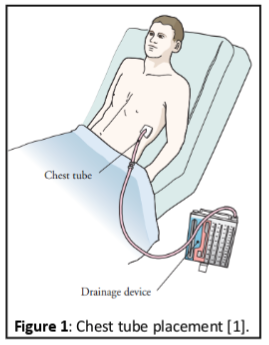
\includegraphics[scale=0.5]{State-art.png}
\end{figure}
\end{columns}
\end{frame}

\begin{frame}[fragile]{Objectives}
\metroset{block=fill}
\begin{alertblock}{Specific Objectives}
\begin{itemize}[<+- | alert@+>]
\item Evaluation of the clinical benefits of the prototype. 
\item Definition and testing of the Good Manufacturing Practices (GMP).  
\item Three material combinations per CTSD part (retainer, base, and receptacle) will be produced. 
\item 100 pre-production prototypes.
\end{itemize}
\end{alertblock}
\end{frame}

\begin{frame}[fragile]{Engineering targets}

% For every picture that defines or uses external nodes, you'll have to
% apply the 'remember picture' style. To avoid some typing, we'll apply
% the style to all pictures.
\tikzstyle{every picture}+=[remember picture]
\tikzstyle{na} = [baseline=-.5ex]

  \begin{columns}[T,onlytextwidth]
    \column{0.5\textwidth}
	\begin{block}{Top part}
	\begin{itemize}
		\item {Flexibility for opening the snaps.} \tikz[na] \coordinate (s-topA);
		\item {Not exceed the maximum elastic zone.} \tikz[na] \coordinate (s-topB);
	\end{itemize}
	\end{block}
	\begin{block}{Bottom part}
	\begin{itemize}
		\item {The adherence with the tape.} \tikz[na] \coordinate (s-topC);
	\end{itemize}
	\end{block}
	\begin{block}{Flexible part}
	\begin{itemize}
		\item Adherence. \tikz[na] \coordinate (s-topD);
		\item Maximum friction. \tikz[na] \coordinate (s-topE);
	\end{itemize}
	\end{block}	
	\column{0.5\textwidth}
	\vspace{2cm}
        % Use a background grid to make it easier to find coordinates
        % When the coordinates have been found, remove the 
        % 'show background grid' option. 
        \tikzstyle{background grid}=[draw, black!50,step=.5cm]
        \begin{tikzpicture}
            % Put the graphic inside a node. This makes it easy to place the
            % graphic and to draw on top of it. 
            % The above right option is used to place the lower left corner
            % of the image at the (0,0) coordinate. 
            \node [inner sep=0pt,above right] 
                {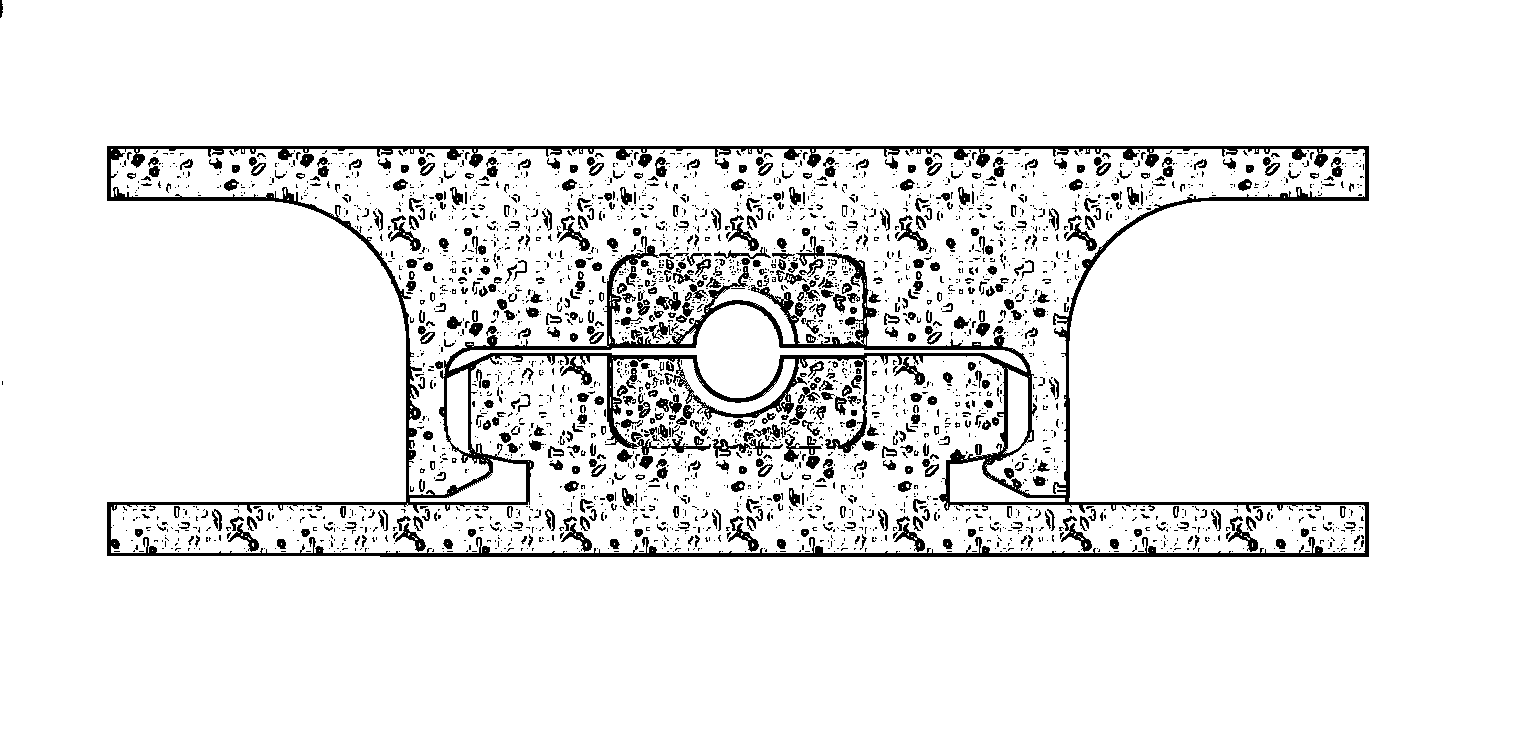
\includegraphics[width=6cm]{chest-tube-flex}};
            % show origin
            \fill[fill=IUcolor] (1.6,1.3) circle (2pt);
            \fill[fill=IUcolor] (1.1,2.2) circle (2pt);
            \fill[fill=IUcolor] (0.5,0.7) circle (2pt);
            \fill[fill=IUcolor] (2.8,1.5) circle (2pt);
            \fill[fill=IUcolor] (2.5,1.2) circle (2pt);
            % define destination coordinates
            \path (1.1,2.2) coordinate (topA)
                  (1.6,1.3) coordinate (topB)
                  (0.5,0.7) coordinate (topC)
                  (2.5,1.2) coordinate (topD)
                  (2.8,1.5) coordinate (topE);
        \end{tikzpicture}
  \end{columns}

\begin{tikzpicture}[overlay]
        \path[->,IUlight,thick] (s-topA) edge [bend left] (topA);
        \path[->,IUlight,thick] (s-topB) edge [bend left] (topB);
        \path[->,IUlight,thick] (s-topC) edge [bend right] (topC);
        \path[->,IUlight,thick] (s-topD) edge [bend right] (topD);
        \path[->,IUlight,thick] (s-topE) edge [bend right] (topE);
\end{tikzpicture}
\end{frame}

% Basically, these are our objectives from the engineering point of view.

\begin{frame}[fragile]{Engineering targets}
\begin{columns}[T,onlytextwidth]
	\column{0.5\textwidth}
	\begin{block}{Whole part}
	\vspace{1cm}
	\begin{itemize}
		\item {The adherence with the rubber part.}
		\item {The product life (fatigue).}
		\item {The proper snap-fit.}
	\end{itemize}
	\end{block}
	\column{0.5\textwidth}
	\begin{figure}
	\vspace{1cm}
	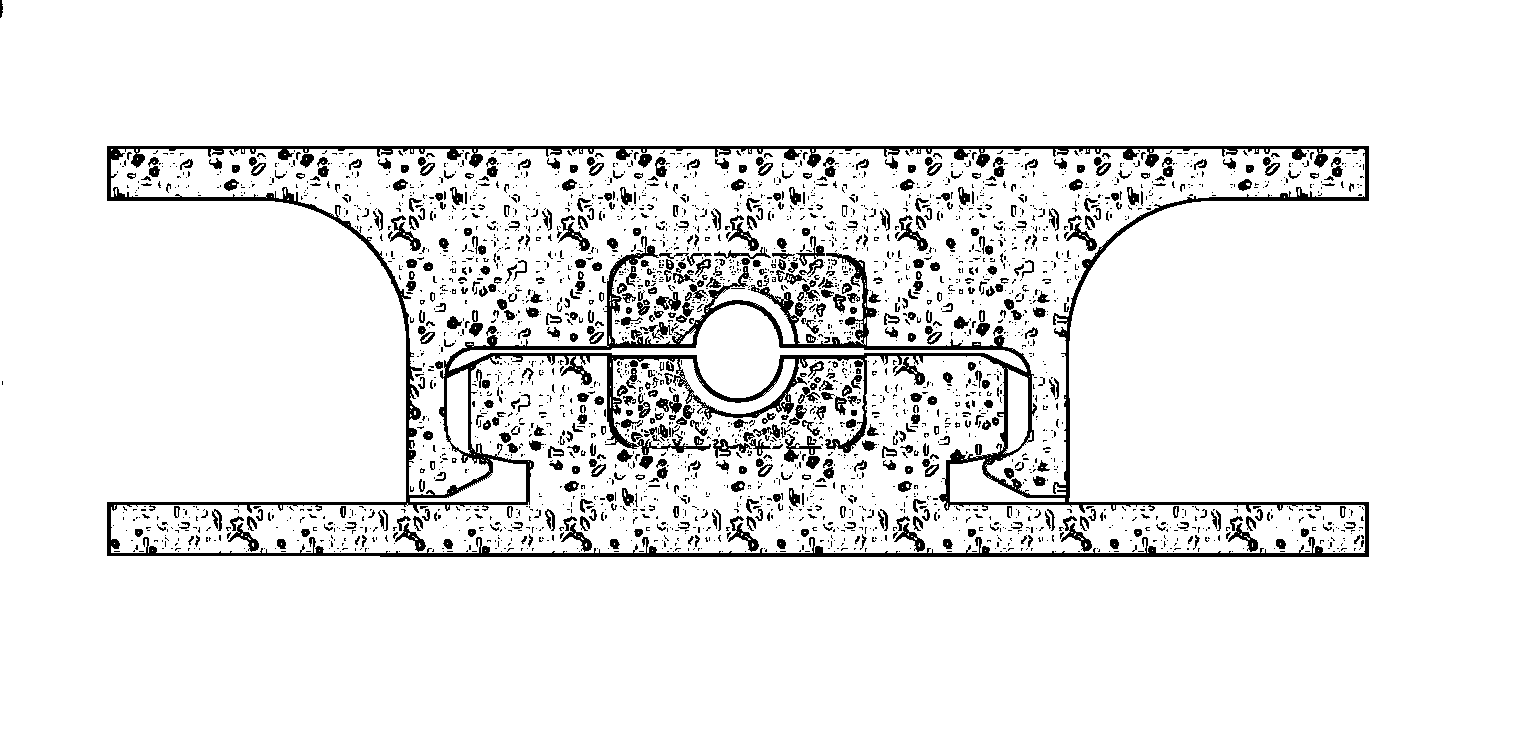
\includegraphics[scale=0.25]{chest-tube-flex}
	\caption{Half-section view complete CTSD}
	\end{figure}
\end{columns}
\end{frame}

\begin{frame}[fragile]{Research Plan}

\begin{alertblock}

According to the design requirements, perform the comparison between 3D printing and plastic injection, in terms of mechanical strength, manufacturing viability, price.  
\end{alertblock}

\metroset{block=transparent}
\begin{block}{Research Plan}
\begin{itemize}[<+- | alert@+>]
\item Evaluation of the 3D printing process.
\item Evaluation of the Plastic injection process. 
\item Numerical analysis process.  
\item Testing protocol.

\end{itemize}
\end{block}
\end{frame}

\section{3D printing process}

\begin{frame}[fragile]{Design of experiments (Part I)}
\begin{table}
\begin{tabular}{|c|c|c|c|c|c|c|c|}
\cline{3-8} 
\multicolumn{1}{c}{} &  & \multicolumn{6}{c|}{Top part}\tabularnewline
\cline{3-8} 
\multicolumn{1}{c}{} &  & ABS & PC/ABS & Nylon & PC & PLA & SLA\tabularnewline
\hline 
\multirow{6}{*}{\rotatebox[origin=c]{90}{Bottom part}} & ABS & \checkmark & \checkmark & \checkmark & \checkmark & \checkmark & \checkmark \tabularnewline
\cline{2-8} 
 & PC/ABS & \checkmark & \checkmark & \checkmark & \checkmark & \checkmark & \checkmark \tabularnewline
\cline{2-8} 
 & Nylon & \checkmark & \checkmark & \checkmark & \checkmark & \checkmark & \checkmark \tabularnewline
\cline{2-8} 
 & PC & \checkmark & \checkmark & \checkmark & \checkmark & \checkmark & \checkmark \tabularnewline
\cline{2-8} 
 & PLA & \checkmark & \checkmark & \checkmark & \checkmark & \checkmark & \checkmark \tabularnewline
\cline{2-8} 
 & SLA & \checkmark & \checkmark & \checkmark & \checkmark & \checkmark & \checkmark \tabularnewline
\hline 
\end{tabular}

\caption{Design of Experiments for 3D printing.}

\end{table}

\end{frame}

\begin{frame}[fragile]{Design of experiments (Part I)}
% Introduce a new counter for counting the nodes needed for circling
\newcounter{nodecount}
% Command for making a new node and naming it according to the nodecount counter
\newcommand\tabnode[1]{\addtocounter{nodecount}{1} \tikz \node (\arabic{nodecount}) {#1};}

\tikzstyle{every picture}+=[remember picture,baseline]
\tikzstyle{every node}+=[inner sep=0pt,anchor=base,
minimum width=0.9cm,align=center,text depth=.25ex,outer sep=1.5pt]
\tikzstyle{every path}+=[thick, rounded corners]
\begin{table}
\begin{tabular}{|c|c|c|c|c|c|c|c|}
\cline{3-8} 
\multicolumn{1}{c}{} &  & \multicolumn{6}{c|}{Top part}\tabularnewline
\cline{3-8} 
\multicolumn{1}{c}{} &  & ABS & PC/ABS & Nylon & PC & PLA & SLA\tabularnewline
\hline 
\multirow{6}{*}{\rotatebox[origin=c]{90}{Bottom part}} & ABS & \checkmark & \checkmark & \checkmark & \checkmark & \checkmark & \tabnode{\checkmark} \tabularnewline
\cline{2-8} 
 & PC/ABS & \tabnode{\checkmark} & \checkmark & \checkmark & \checkmark & \checkmark & \checkmark \tabularnewline
\cline{2-8} 
 & Nylon & \checkmark & \tabnode{\checkmark} & \checkmark & \checkmark & \checkmark & \checkmark \tabularnewline
\cline{2-8} 
 & PC & \checkmark & \checkmark & \tabnode{\checkmark} & \checkmark & \checkmark & \checkmark \tabularnewline
\cline{2-8} 
 & PLA & \checkmark & \checkmark & \checkmark & \tabnode{\checkmark} & \checkmark & \checkmark \tabularnewline
\cline{2-8} 
 & SLA & \tabnode{\checkmark} & \checkmark & \checkmark & \checkmark & \checkmark & \tabnode{\checkmark} \tabularnewline
\hline 
\end{tabular}
\caption{Full factorial DOE for 3D printing.}
\begin{tikzpicture}[overlay]
% Define the circle paths
\draw [orange] (2.north west) -- (2.north east) -- (2.south east) -- (3.north west) -- (3.north east) -- (3.south east) -- (4.north west) -- (4.north east) -- (4.south east) -- (5.north west) -- (5.north east) -- (5.south east) -- (7.north west) -- (7.south west) -- (6.south west) -- cycle;
\draw [red] (1.north west) -- (1.north east) -- (7.north east) -- (7.north west) -- cycle;  
\end{tikzpicture}

\end{table}

\end{frame}

\begin{frame}[fragile]{Design of experiments (Part I)}
\begin{table}
\begin{tabular}{|c|c|c|c|c|c|c|c|}
\cline{3-8} 
\multicolumn{1}{c}{} &  & \multicolumn{6}{c|}{Top part}\tabularnewline
\cline{3-8} 
\multicolumn{1}{c}{} &  & ABS & PC/ABS & Nylon & PC & PLA & SLA\tabularnewline
\hline 
\multirow{6}{*}{\rotatebox[origin=c]{90}{Bottom part}} & ABS & \checkmark & \checkmark & \checkmark & \checkmark & \checkmark & \tabularnewline
\cline{2-8} 
 & PC/ABS &  & \checkmark & \checkmark & \checkmark & \checkmark & \tabularnewline
\cline{2-8} 
 & Nylon & & & \checkmark & \checkmark & \checkmark & \tabularnewline
\cline{2-8} 
 & PC & & & & \checkmark & \checkmark &  \tabularnewline
\cline{2-8} 
 & PLA & & & & & \checkmark &  \tabularnewline
\cline{2-8} 
 & SLA & & & & & & \checkmark \tabularnewline
\hline 
\end{tabular}

\caption{Total number of combinations.}

\end{table}

\end{frame}

\begin{frame}[fragile]{Flexible part}

\begin{columns}[T,onlytextwidth]
\column{0.5\textwidth}
\begin{table}
\begin{tabular}{|l|l|}
\hline
Flexible materials & Printing Method \\ \hline
TPE                & FDM             \\ \hline
TPU                & FDM             \\ \hline
Flexible           & SLA             \\ \hline
\end{tabular}
\end{table}
\column{0.5\textwidth}
\begin{figure}
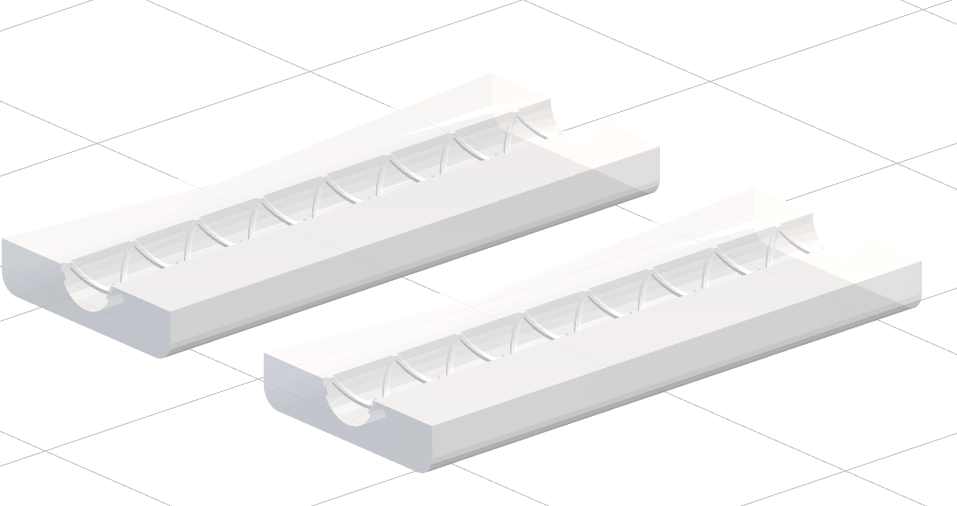
\includegraphics[scale=0.25]{receptacle}
\caption{Receptacle CAD}
\end{figure}
\end{columns}
\end{frame}

\begin{frame}[fragile]{Total number of experiments}
\vspace{1cm}
\begin{columns}[T,onlytextwidth]
\column{0.5\textwidth}
\begin{table}
\begin{centering}
\begin{tabular}{|c|c|}
\hline 
ID & No.\tabularnewline
\hline 
\hline 
Top - Base & 16\tabularnewline
\hline 
Flexible & 3\tabularnewline
\hline 
Total & 48\tabularnewline
\hline 
\end{tabular}
\par\end{centering}
\caption{Total Number of experiments}
\end{table}
\column{0.5\textwidth}
\begin{figure}
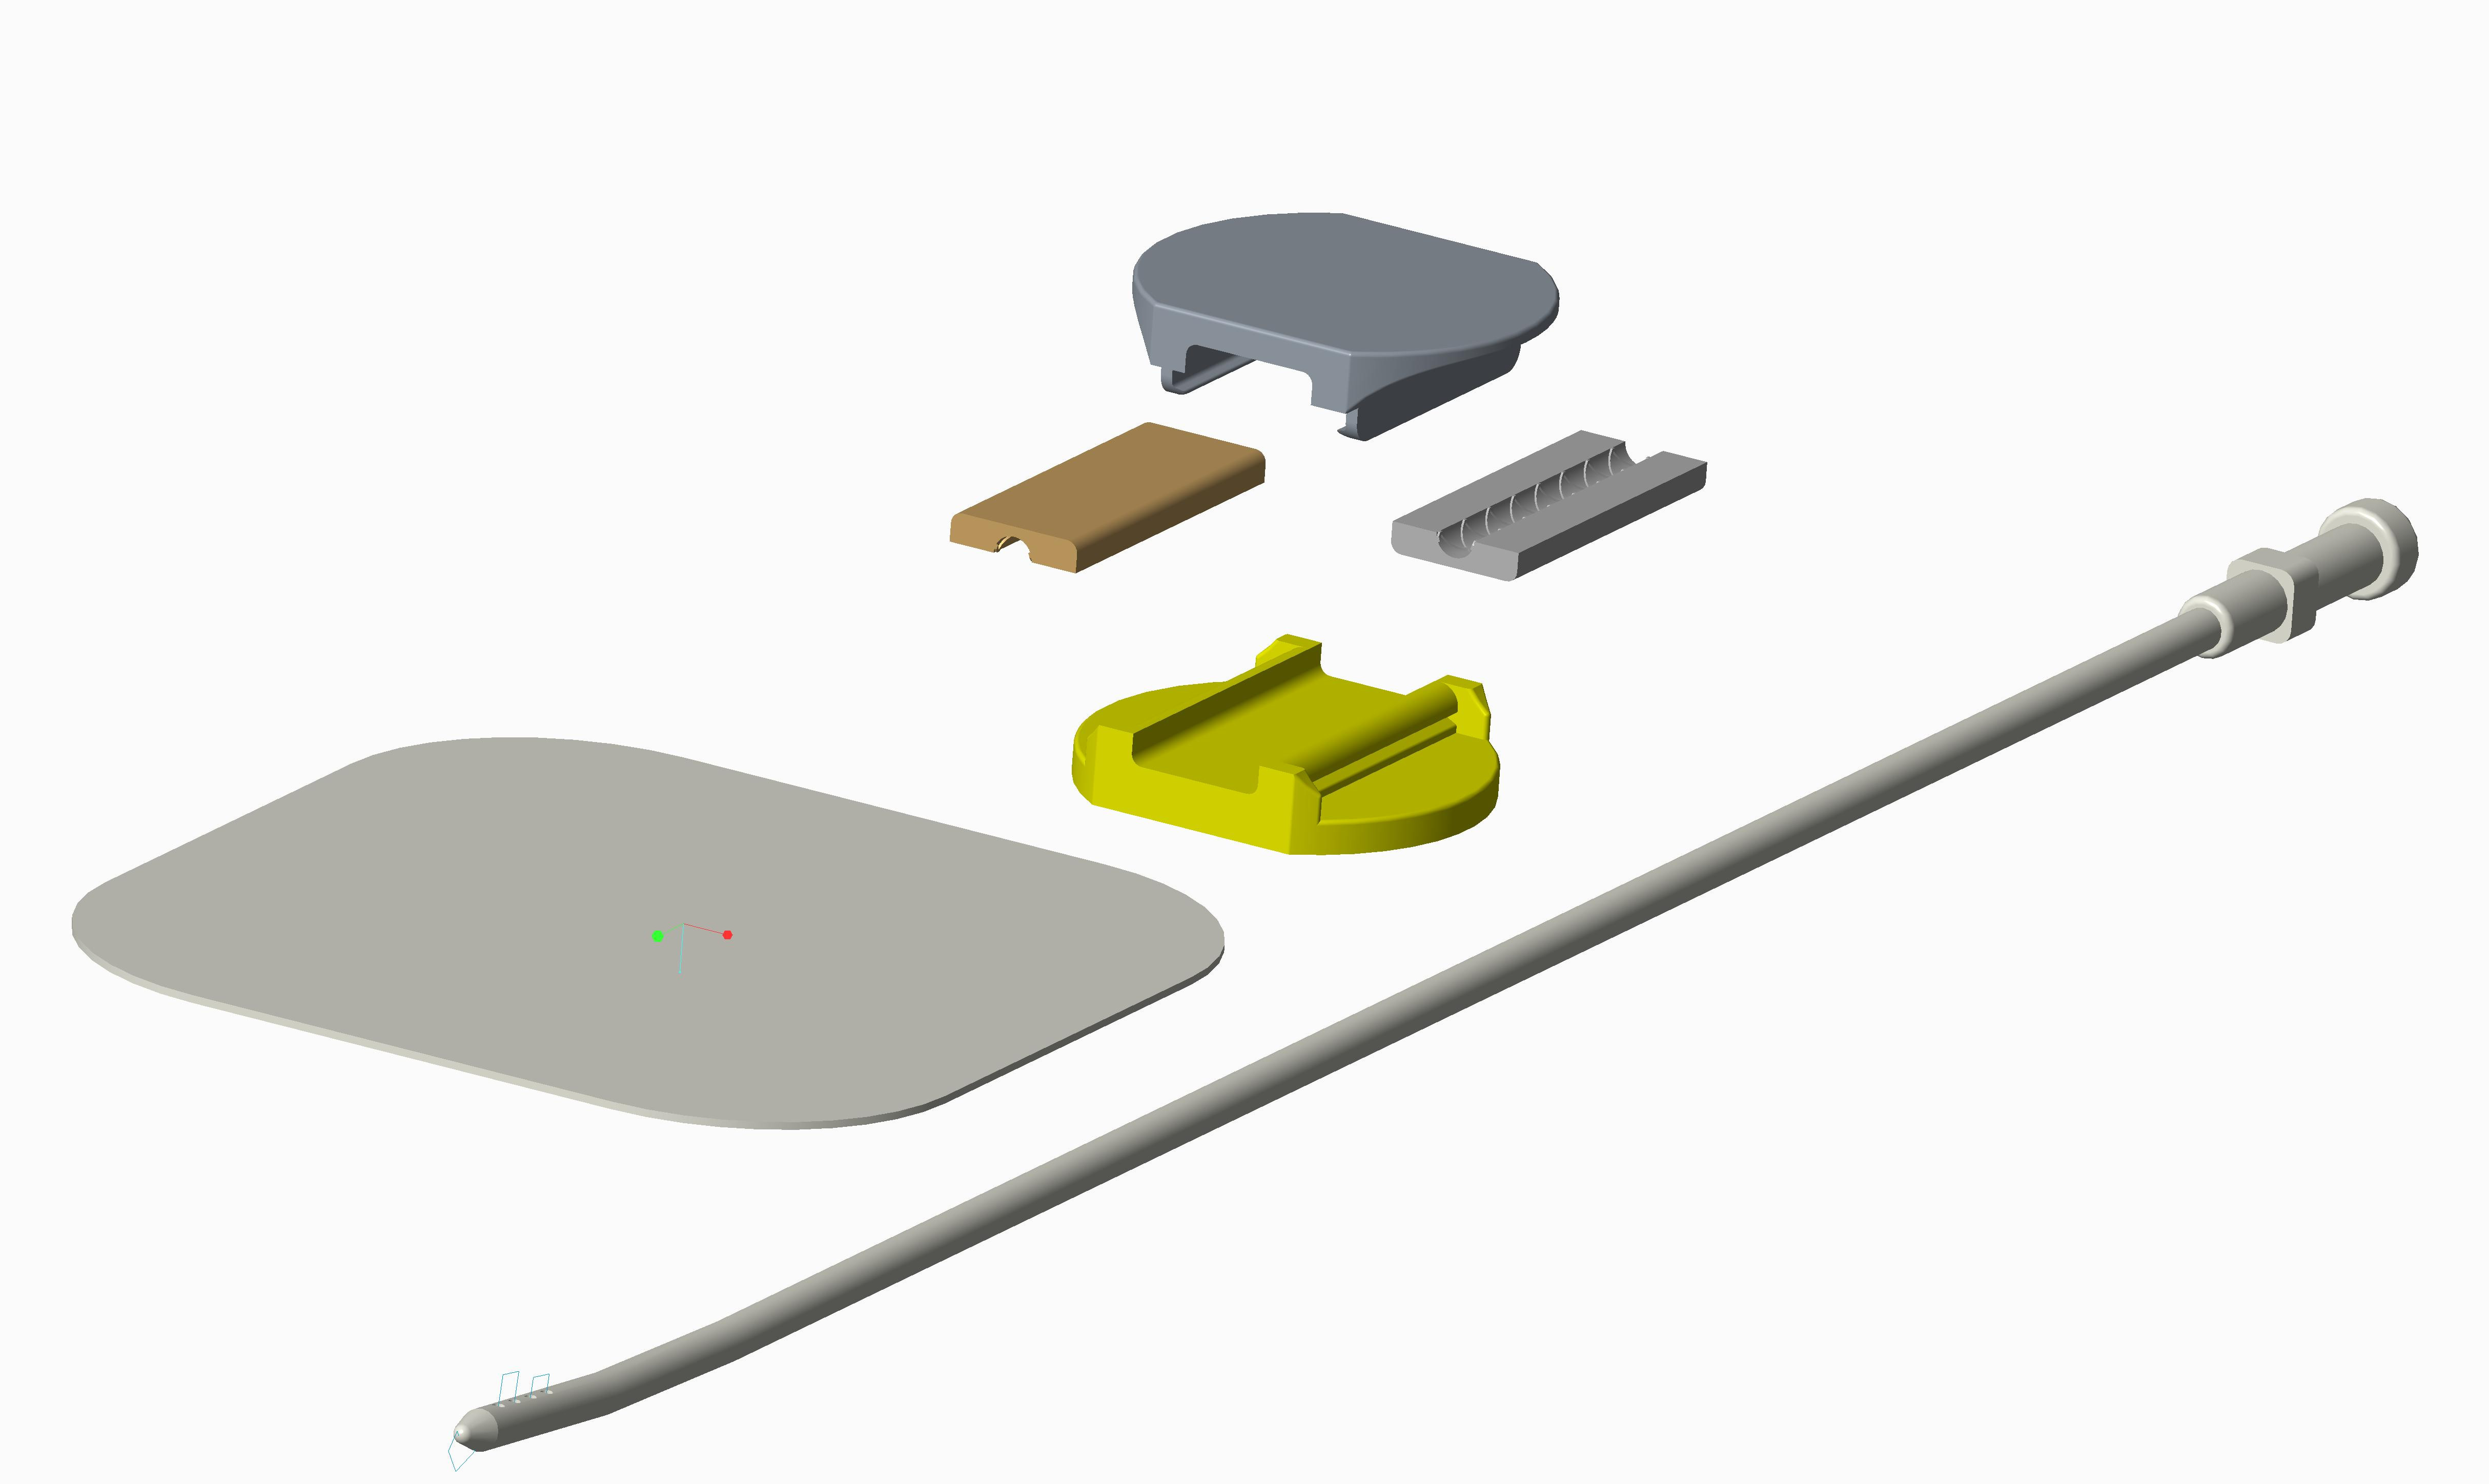
\includegraphics[scale=0.025]{chesttube}
\caption{Render of the CTSD}
\end{figure}
\end{columns}
\end{frame}

\begin{frame}[fragile]{What do we want to figure out?}	
\begin{columns}[T,onlytextwidth]
\column{0.5\textwidth}
\begin{block}{Manufacturability}
\begin{itemize}
\item Printing quality.
\item Time.
\item Printing complexity.
\end{itemize}
\end{block}
\begin{block}{Mechanical properties}
\begin{itemize}
\item Bonding force.
\item Sliding force.
\item Snapping.
\end{itemize}
\end{block}
\column{0.5\textwidth}
\begin{figure}
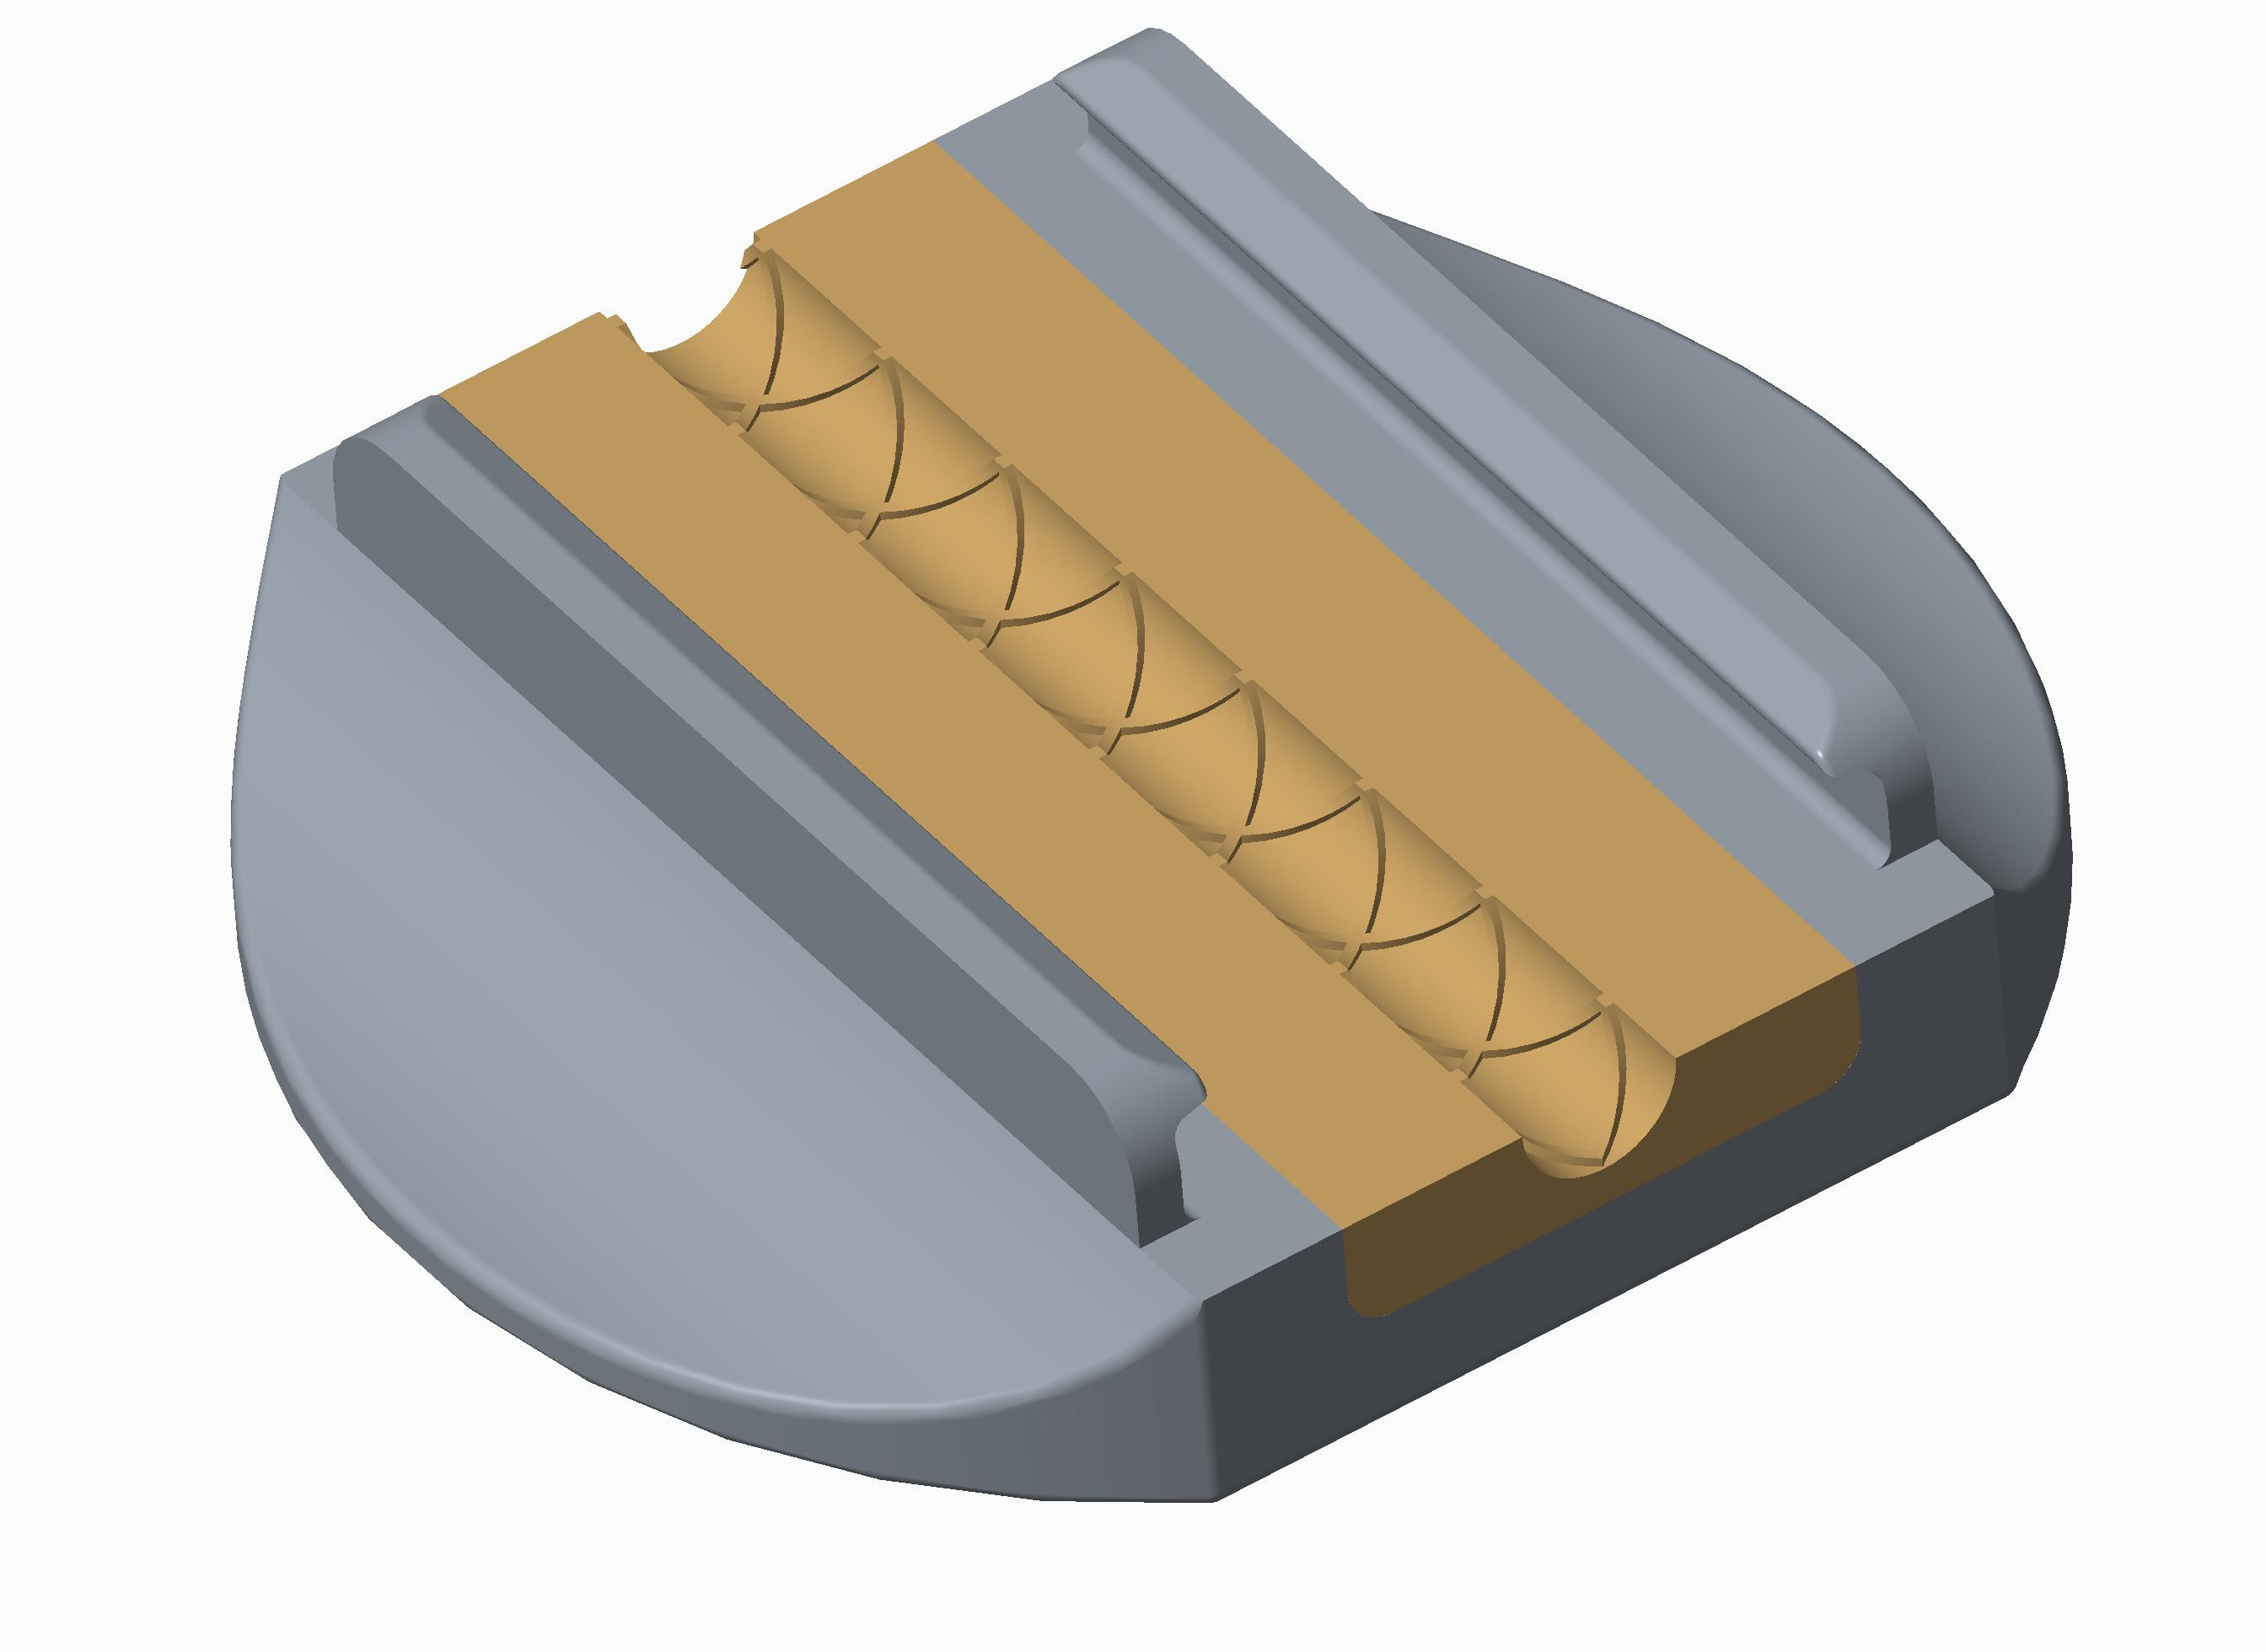
\includegraphics[scale=0.04]{chesttube_top}
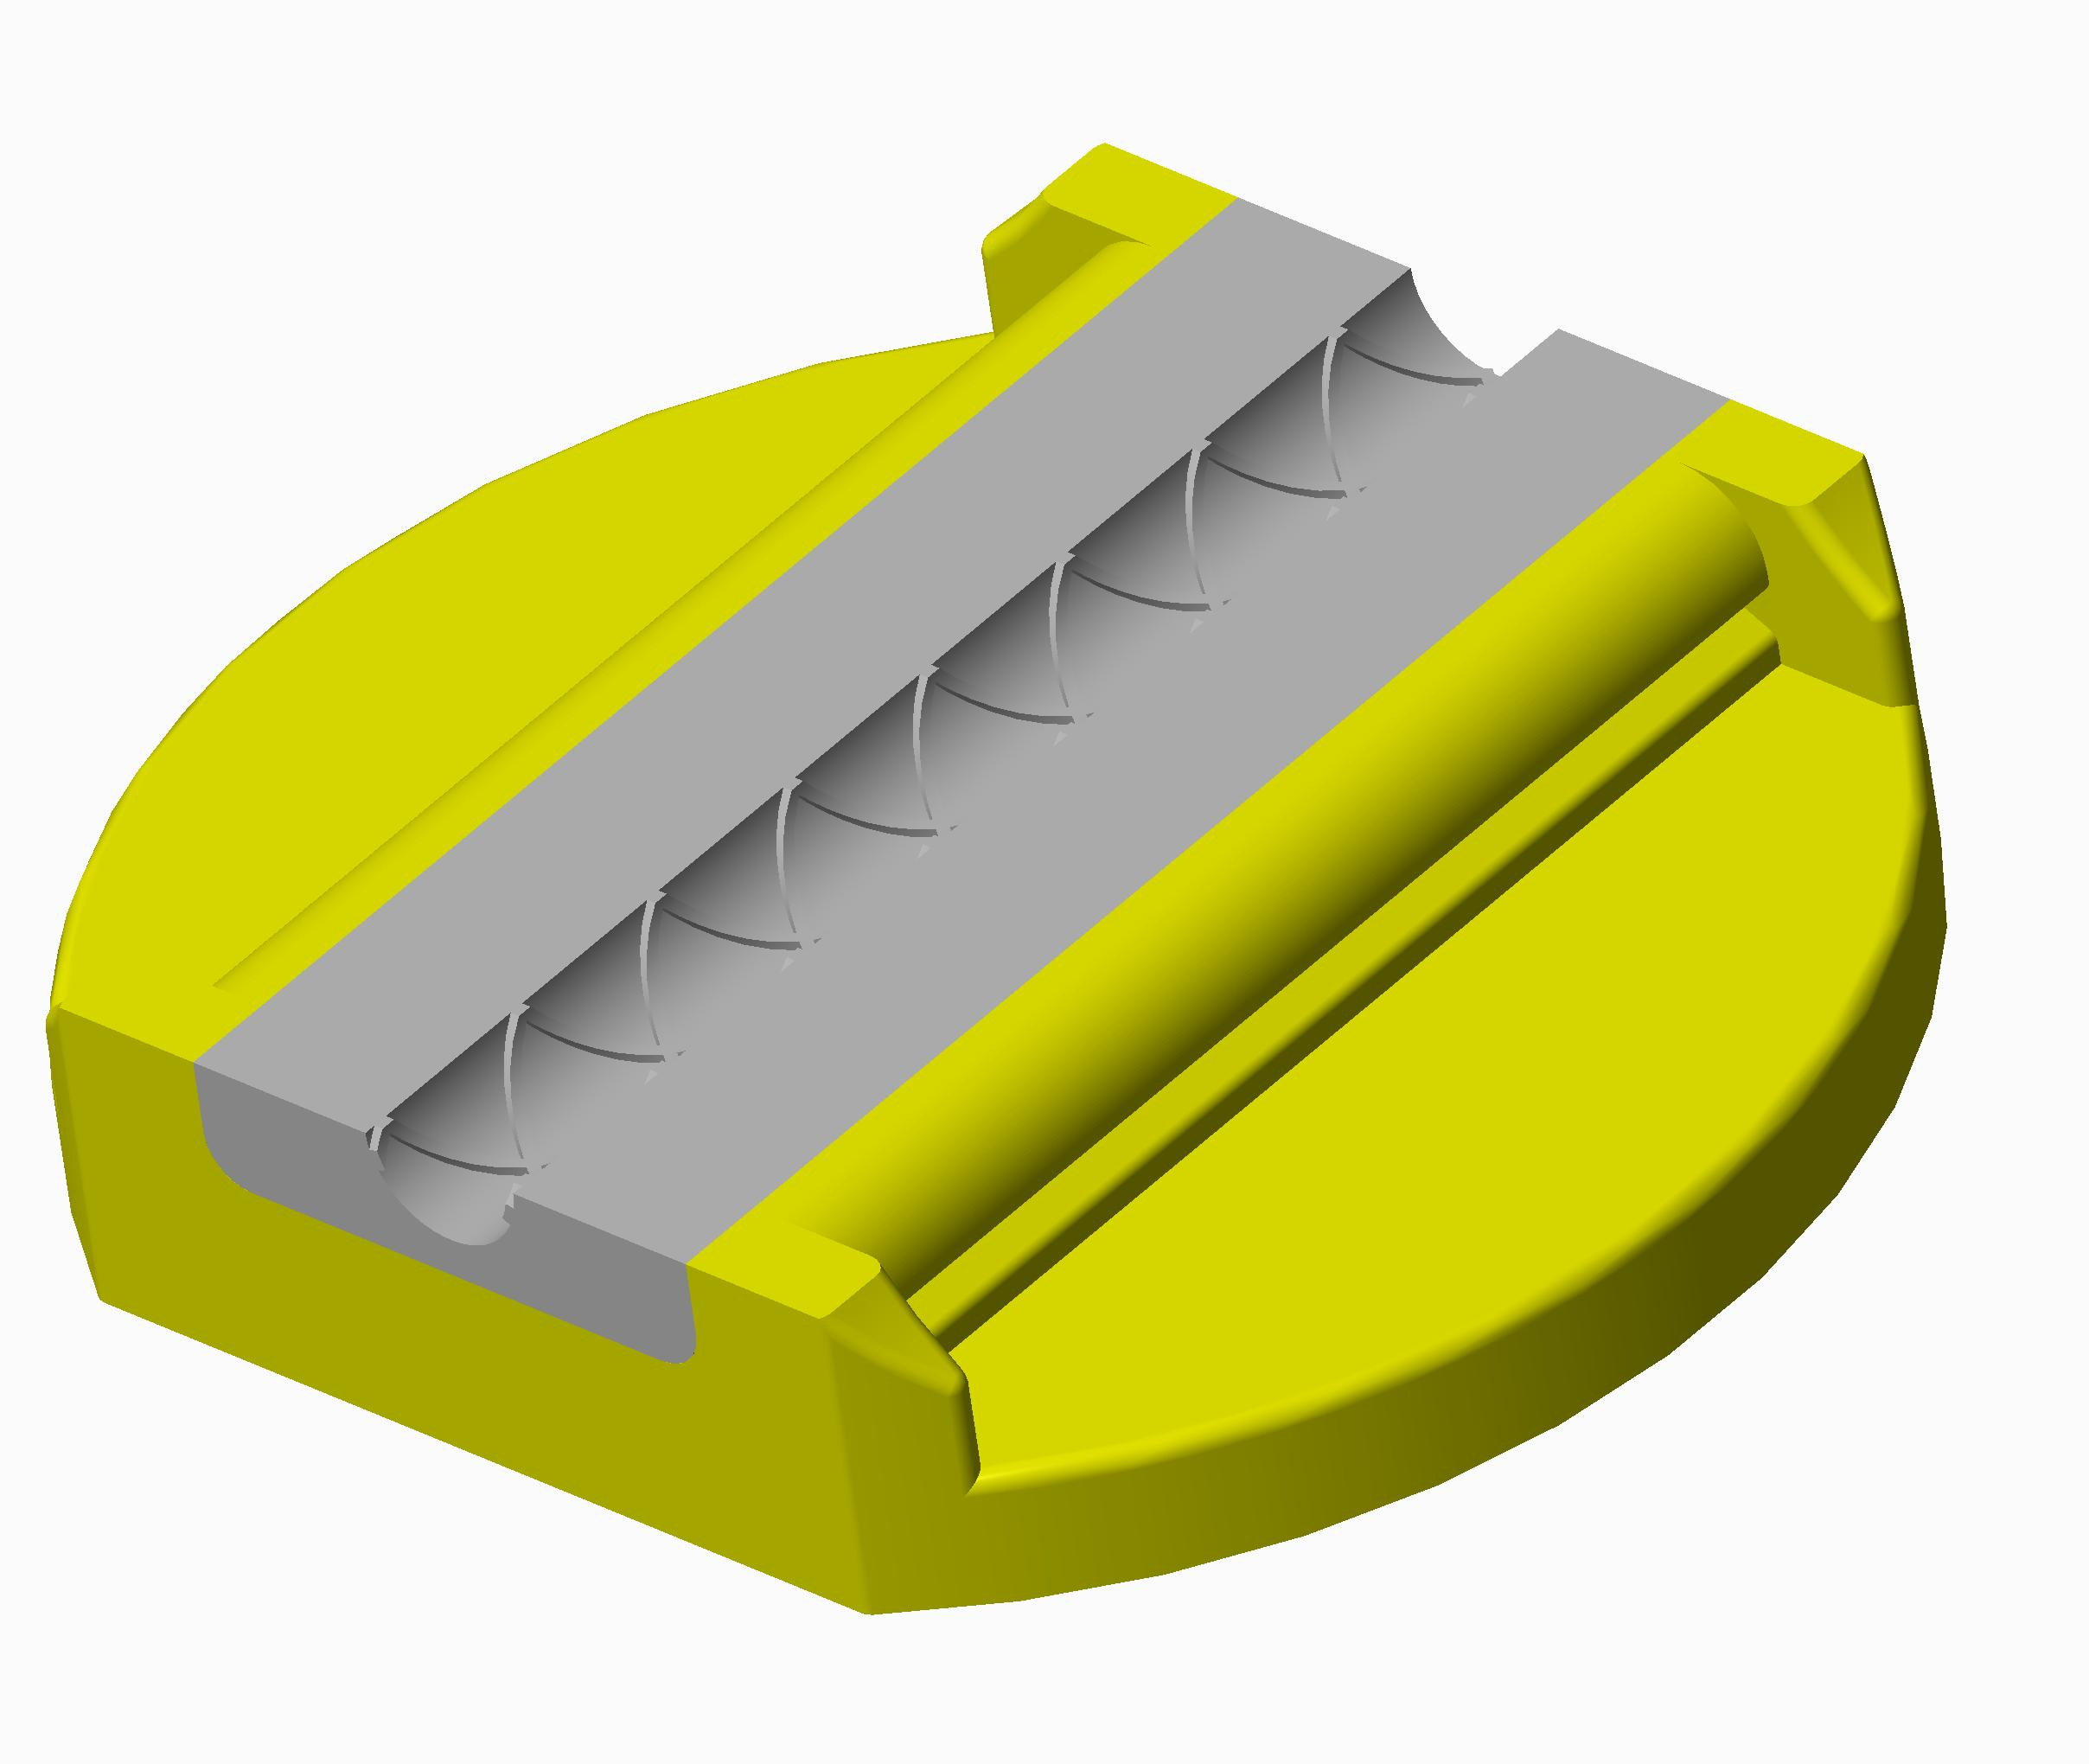
\includegraphics[scale=0.04]{chesttube_base}
\caption{Dual material parts render.}
\end{figure}
\end{columns}
\end{frame}

\section{Plastic Injection Molding}
\begin{frame}[fragile]{Design mold process}
\smartdiagramset{border color=none,
uniform color list=IUlight for 4 items,
arrow style=[-stealth’,
module x sep=5,
back arrow distance=0.75,
priority arrow height advance=1.0cm
}
\smartdiagram[priority descriptive diagram]{
  Choose the material according to the 3D print experiment, 
  Make molds in 3D printing,
  Develop the dual injecting process,  
  Develop the final mold 
  }
\end{frame}

\begin{frame}[fragile]{Methodology}
\begin{center}
\smartdiagramset{planet color=IUcolor,
distance planet-satellite=2.8cm
}
\smartdiagram[circular diagram:clockwise]
{Simulate Physical Parameters, Build a 3D print mold, Set up the process, Run, Analyze, Modify~/\\ Add,Check}
\end{center}
\end{frame}
\section{Numerical Analysis process}
\begin{frame}[fragile]{Finite Element Analysis}
\begin{columns}[T,onlytextwidth]
	\column{0.5\textwidth}
	\begin{block}{Purpose I}
	\begin{itemize}
		\item {To determine max stresses.}
		\item {To determine the product life (fatigue).}
		\item {To make structural optimization.}
	\end{itemize}
	\end{block}
	\begin{block}{Purpose II}
	\begin{itemize}
		\item {CTSD experiments.}
		\item {To avoid mold trials.}
	\end{itemize}
	\end{block}
	\column{0.5\textwidth}
	\begin{figure}
	\vspace{1cm}
	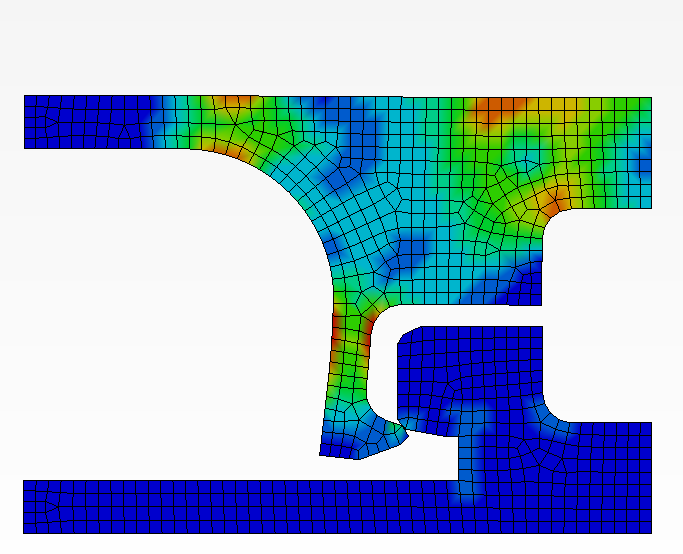
\includegraphics[scale=0.25]{CTSDsimulation}
	\caption{Explicit Simulation CTSD}
	\end{figure}
\end{columns}
\end{frame}

\section{Testing process}

\begin{frame}[fragile]{Sliding force}
\begin{columns}[T,onlytextwidth]
\column{0.5\textwidth}
\metroset{block=fill}
	\begin{figure}
	\vspace{1cm}
	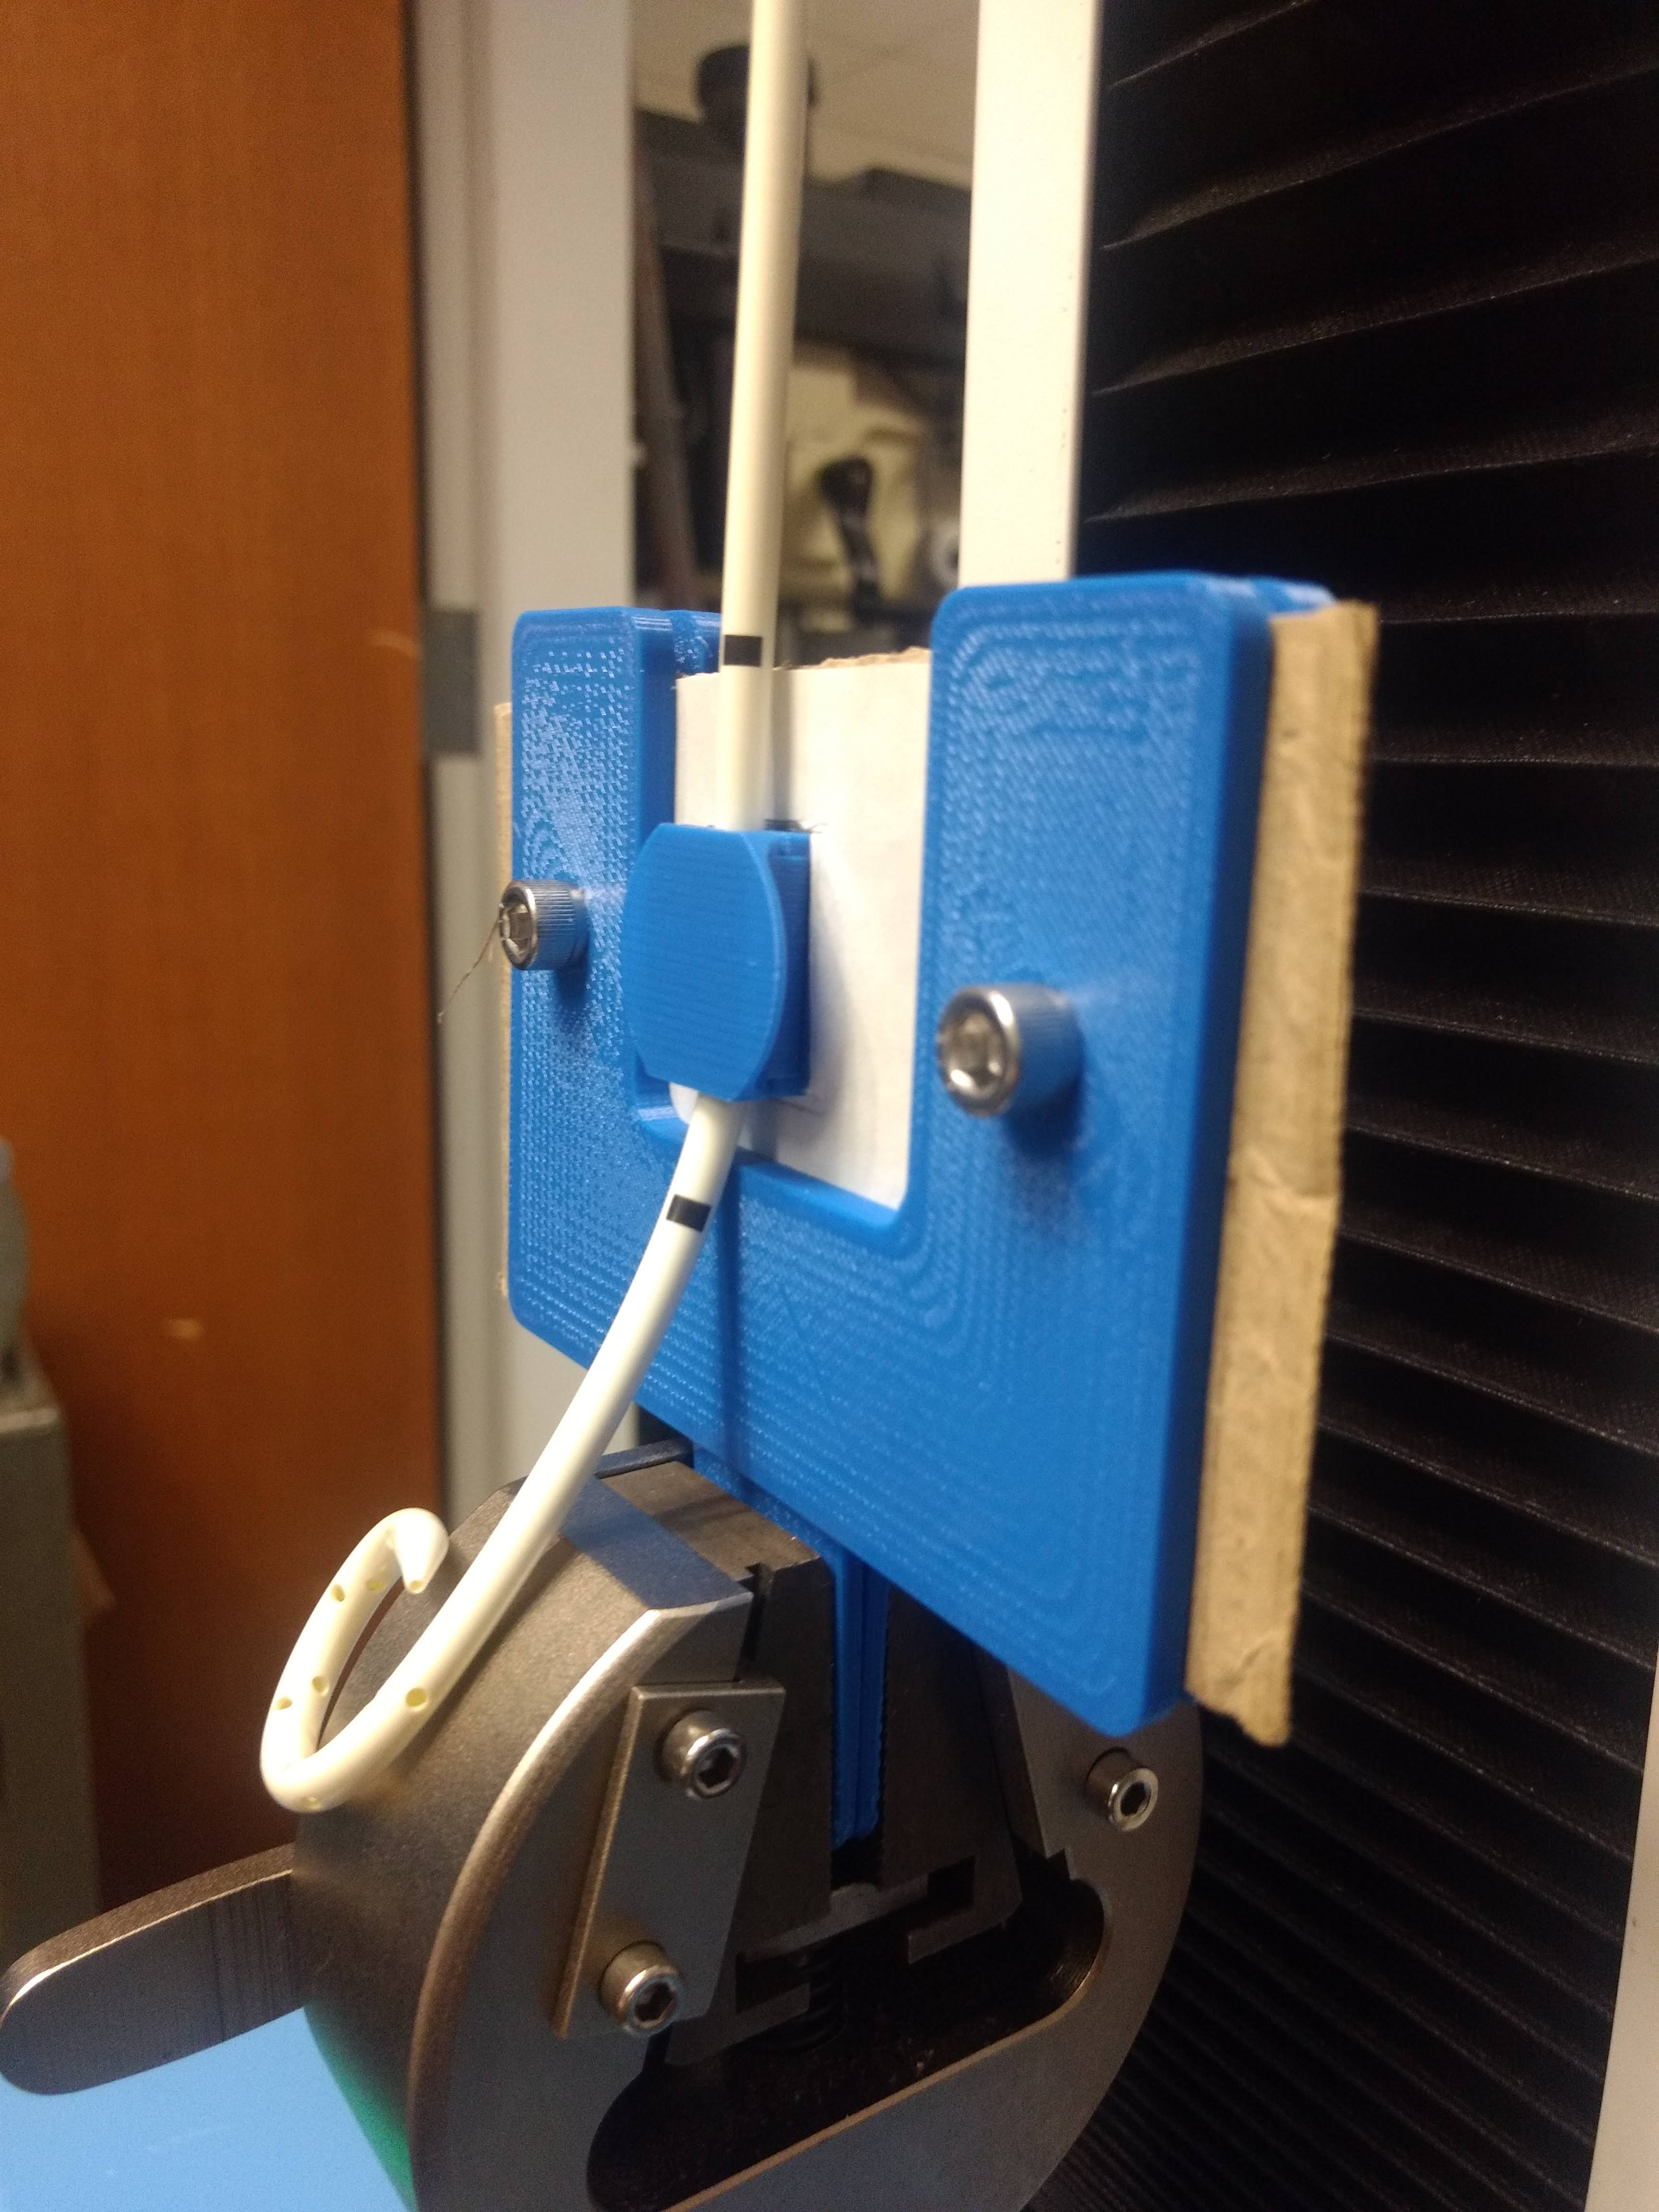
\includegraphics[scale=0.03]{test-CTHD}
	\caption{Sliding force testing.}
	\end{figure}
\column{0.5\textwidth}
	\begin{figure}
	\vspace{1cm}
	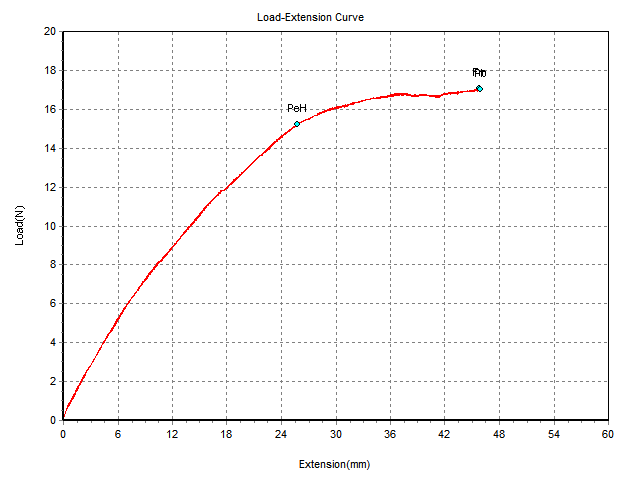
\includegraphics[scale=0.5]{Test1ChestHold}
	\caption{Force Displacement curvature}
	\end{figure}
\end{columns}
\end{frame}

{%

\section{Schedule}
\begin{frame}[fragile]{Schedule}

\begin{ganttchart}[
time slot format=isodate-yearmonth,
x unit=1.0cm,
y unit title=0.7cm,
y unit chart=0.8cm,
vgrid,
time slot unit=month,
%compress calendar,
title/.append style={draw=none, fill=IUcolor},
title label font=\footnotesize\sffamily\bfseries\color{white},
title label node/.append style={below=-1.6ex},
title left shift=.05,
title right shift=-.05,
title height=1,
bar/.append style={draw=none, fill=green!75},
bar height=.6,
bar label font=\normalsize\color{black!50},
group right shift=0,
group top shift=.6,
group height=.3,
group peaks height=.2,
bar incomplete/.append style={fill=IUlight},
]{2018-07}{2018-12}
%\gantttitlecalendar{year}{months} \\
\gantttitle[]{2018}{5} \\                 % title 
	\gantttitle{Aug}{1}
    \gantttitle{Sep}{1}
    \gantttitle{Oct}{1}
    \gantttitle{Nov}{1}
    \gantttitle{Dic}{1}\\
\ganttset{progress label text={}, link/.style={black, -to}}
\ganttgroup{Pre-manufacturing Line}{2018-07}{2018-12}\\ 
\ganttbar[progress=10, name=T1A]{3D printing experiment.}{2018-07}{2018-10} \\
\ganttbar[progress=0, name=T1A]{Testing 3D printing}{2018-09}{2018-10} \\
\ganttbar[progress=0, name=T1A]{Injection Molding}{2018-09}{2018-11} \\
\ganttbar[progress=0, name=T1A]{Testing IM prototypes}{2018-10}{2018-12} \\
\ganttbar[progress=0, name=T1A]{Preparing one journal paper.}{2018-08}{2018-12} \\
\ganttset{link/.style={black}}
%\ganttlink[link mid=.4]{pp}{T1A}
%\ganttlink[link mid=.159]{pp}{T2A}
\end{ganttchart}
\end{frame}
{\setbeamercolor{palette primary}{fg=black, bg=yellow}
\begin{frame}[standout]
  Questions?
\end{frame}
}

%\appendix


%\begin{frame}[allowframebreaks]{References}

%  \bibliography{demo}
%  \bibliographystyle{abbrv}

%\end{frame}

\end{document}
